% Compile with latex to get .div output
% Then execute dvisvgm to convert .div to .svg, use --no-fonts if fonts go wrong.
\documentclass[tikz]{standalone}
\usetikzlibrary{arrows.meta,positioning,automata}
\begin{document}
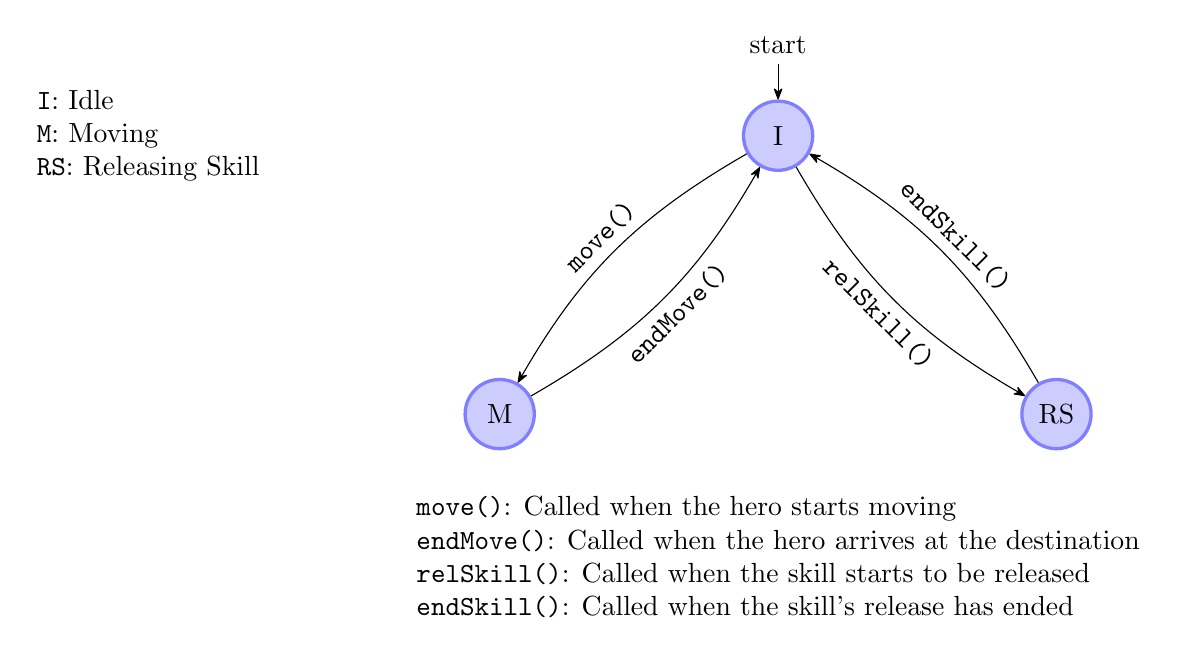
\begin{tikzpicture}[%
	node distance=5cm,on grid,>={Stealth[round]},
	every state/.style={draw=blue!50,very thick,fill=blue!20},
	initial where=above]
	
	\node (TXT) [align=left] {%
		\texttt{I}: Idle\\
		\texttt{M}: Moving\\
		\texttt{RS}: Releasing Skill
	};

	\node[state,initial]	(I)	[right=8cm of TXT]	{I};
	\node[state]			(M)	[below left=of I]	{M};
	\node[state]			(RS)[below right=of I]	{RS};


	\path[->] (I)  edge [bend right=15]	node	[sloped,above]	{\texttt{move()}}
		(M);
	\path[->] (M)  edge [bend right=15]	node	[sloped,below]	{\texttt{endMove()}}
		(I);
	\path[->] (I)  edge [bend right=15]	node	[sloped,below]	{\texttt{relSkill()}}
		(RS);
	\path[->] (RS) edge [bend right=15]	node	[sloped,above]	{\texttt{endSkill()}}
		(I);

	\node [anchor=north,below=4cm of I.south,align=left] {%
		\texttt{move()}: Called when the hero starts moving\\
		\texttt{endMove()}: Called when the hero arrives at the destination\\
		\texttt{relSkill()}: Called when the skill starts to be released\\
		\texttt{endSkill()}: Called when the skill's release has ended
	};

\end{tikzpicture}
\end{document}